\chapter{Dissolving Ionic and Molecular Solids}\label{ch:g11:dissolution}

A pinch of salt stirred into water vanishes in seconds; the same pinch
stirred into cooking oil lies at the bottom of the glass, unchanged, for
as long as anyone cares to watch. A greasy pan rinsed under the tap stays
greasy; one drop of washing-up liquid, and the grease lifts off. What
decides whether a substance \omterm{def:g2:mixing-and-dissolving:dissolve}{dissolves} in a liquid? The answer lies in
the \omterm{def:g11:polarity-and-cohesion:polar-bond}{partial charges} and the forces between particles of the previous
chapter.

\begin{recall}
\omterm{def:g6:solutions-and-solubility:solubility}{Solubility}; \omterm{def:g6:solutions-and-solubility:miscible}{miscible} and \omterm{def:g6:solutions-and-solubility:miscible}{immiscible} liquids
(\cref{ch:g6:solutions-and-solubility}). An \omterm{def:g9:ions:ionic-compound}{ionic compound} is made of
\omterm{def:g9:ions:ion}{cations} and \omterm{def:g9:ions:ion}{anions} in proportions that make it neutral
(\cref{ch:g9:ions}). Polar and \omterm{def:g11:polarity-and-cohesion:polar-molecule}{non-polar molecules}, \omterm{def:g11:polarity-and-cohesion:hydrogen-bond}{hydrogen bonds},
\omterm{def:g11:polarity-and-cohesion:van-der-waals}{van der Waals interactions} (\cref{ch:g11:polarity-and-cohesion}).
\omterm{def:g10:chemical-species:extraction}{Liquid--liquid extraction} (\cref{ch:g10:chemical-species}). \omterm{def:g10:concentration-and-dilution:molar-concentration}{Molar
concentration} (\cref{ch:g10:concentration-and-dilution}).
\end{recall}

\section{Dissolving an ionic solid}

In a crystal of sodium chloride, each sodium \omterm{def:g9:ions:ion}{ion} \ce{Na+} is surrounded
by chloride \omterm{def:g9:ions:ion}{ions} \ce{Cl-} and each chloride \omterm{def:g9:ions:ion}{ion} by sodium \omterm{def:g9:ions:ion}{ions}, all held
by the attraction between opposite charges. Water \omterm{def:g7:atoms-and-molecules:molecule}{molecules}, polar, are
attracted by these charges: their oxygen side ($\delta^-$) turns towards
the \omterm{def:g9:ions:ion}{cations}, their hydrogen side ($\delta^+$) towards the \omterm{def:g9:ions:ion}{anions}.

\begin{definition}[Dissociation]\label{def:g11:dissolution:dissociation}
The \emph{dissociation}\index{dissociation} of an ionic solid in a
\omterm{def:g6:solutions-and-solubility:solute}{solvent} is the separation of its \omterm{def:g9:ions:ion}{ions} from one another: they leave the
crystal and move apart in the solution.
\end{definition}

\begin{definition}[Solvation, hydration]\label{def:g11:dissolution:solvation}
The \emph{solvation}\index{solvation} of a dissolved particle is its
surrounding by \omterm{def:g6:solutions-and-solubility:solute}{solvent} \omterm{def:g7:atoms-and-molecules:molecule}{molecules}, held to it by attractions; in water it
is called \emph{hydration}\index{hydration}. The symbol (aq) after a
formula means ``hydrated''.
\end{definition}

\begin{proposition}[Three stages of dissolving]\label{prop:g11:dissolution:stages}
An ionic solid \omterm{def:g2:mixing-and-dissolving:dissolve}{dissolves} in water in three stages that happen together:
the \omterm{def:g9:ions:ion}{ions} are pulled out of the crystal (\omterm{def:g11:dissolution:dissociation}{dissociation}), surrounded by
water \omterm{def:g7:atoms-and-molecules:molecule}{molecules} (\omterm{def:g11:dissolution:solvation}{hydration}), and spread through the whole solution
(dispersion). For sodium chloride,
\[
  \ce{NaCl(s) -> Na+(aq) + Cl-(aq)} .
\]
\end{proposition}

\begin{proof}
Admitted: the attractions between the \omterm{def:g9:ions:ion}{ions} and the polar water
\omterm{def:g7:atoms-and-molecules:molecule}{molecules}, added up, are strong enough to replace those between the
\omterm{def:g9:ions:ion}{ions} of the crystal.
\end{proof}

\begin{omfigure}
\begin{tikzpicture}[font=\small]
  % the crystal edge: alternating ions
  \foreach \i in {0,1,2,3,4} \foreach \j in {0,1,2,3} {
    \pgfmathtruncatemacro\k{mod(\i+\j,2)}
    \ifnum\k=0
      \node[om atom, ball color=green!60!black, minimum size=6.4mm] at (0.8*\i,0.8*\j) {};
    \else
      \node[om atom, ball color=violet!70, minimum size=4.0mm] at (0.8*\i,0.8*\j) {};
    \fi
  }
  % a hydrated Na+ that has left: O towards the ion
  \begin{scope}[shift={(5.6,1.8)}]
    \node[om atom, ball color=violet!70, minimum size=4.0mm] (na) at (0,0) {};
    \node[font=\footnotesize] at (0,0) {};
    \foreach \a in {0,90,180,270} {
      \node[aO, minimum size=4.6mm] (o\a) at (\a:0.62) {};
      \node[aH, minimum size=3.2mm] (ha\a) at ($(\a:0.62)+(\a+52:0.42)$) {};
      \node[aH, minimum size=3.2mm] (hb\a) at ($(\a:0.62)+(\a-52:0.42)$) {};
      \begin{scope}[on background layer]
        \draw[bond, line width=1.2pt] (o\a.center) -- (ha\a.center);
        \draw[bond, line width=1.2pt] (o\a.center) -- (hb\a.center);
      \end{scope}
    }
    \node[anchor=north] at (0,-1.35) {\ce{Na+(aq)}};
  \end{scope}
  % a hydrated Cl- that has left: H towards the ion
  \begin{scope}[shift={(8.6,1.4)}]
    \node[om atom, ball color=green!60!black, minimum size=6.4mm] at (0,0) {};
    \foreach \a in {45,135,225,315} {
      \node[aH, minimum size=3.2mm] (h\a) at (\a:0.62) {};
      \node[aO, minimum size=4.6mm] (o\a) at (\a:1.0) {};
      \node[aH, minimum size=3.2mm] (k\a) at ($(\a:1.0)+(\a+75:0.42)$) {};
      \begin{scope}[on background layer]
        \draw[bond, line width=1.2pt] (o\a.center) -- (h\a.center);
        \draw[bond, line width=1.2pt] (o\a.center) -- (k\a.center);
      \end{scope}
    }
    \node[anchor=north] at (0,-1.45) {\ce{Cl-(aq)}};
  \end{scope}
  \node[anchor=north, align=center] at (1.6,-0.45) {the crystal\\
    (\ce{Na+} small, \ce{Cl-} large)};
\end{tikzpicture}

{\small Sodium chloride dissolving. A sodium \omterm{def:g9:ions:ion}{ion} and a chloride \omterm{def:g9:ions:ion}{ion} have
left the crystal; each is hydrated. Around the \omterm{def:g9:ions:ion}{cation} the water \omterm{def:g7:atoms-and-molecules:molecule}{molecules}
turn their oxygen \omterm{def:g7:atoms-and-molecules:atom}{atoms} (red, $\delta^-$) inwards, around the \omterm{def:g9:ions:ion}{anion} their
hydrogen \omterm{def:g7:atoms-and-molecules:atom}{atoms} (white, $\delta^+$).}
\end{omfigure}

\section{Concentrations of the ions}

\begin{method}[Concentration of each ion]\label{met:g11:dissolution:ions}
\begin{enumerate}
  \item Write the dissolution equation, balanced in \omterm{def:g7:atoms-and-molecules:atom}{atoms} and in charge:
        for calcium chloride, \ce{CaCl2(s) -> Ca^{2+}(aq) + 2Cl-(aq)}.
  \item Compute the amount $n$ of solid dissolved, and the concentration
        $c = n / V$ of the solution in \omterm{def:g6:solutions-and-solubility:solute}{solute}.
  \item Each \omterm{def:g9:ions:ion}{ion} has the concentration $c$ multiplied by its coefficient
        in the equation: here $[\ce{Ca^{2+}}] = c$ and
        $[\ce{Cl-}] = 2c$.
\end{enumerate}
The square brackets $[\ldots]$ denote the \omterm{def:g10:concentration-and-dilution:molar-concentration}{molar concentration} of a
dissolved species.
\end{method}

\begin{example}[Calcium chloride]\label{ex:g11:dissolution:cacl2}
% ledger: aw:Ca, aw:Cl
\qty{5.55}{g} of calcium chloride ($M = \qty{111.1}{g/mol}$) dissolved
to make \qty{500.0}{mL} of solution: $n = \qty{0.0500}{mol}$,
$c = \qty{0.100}{mol/L}$, so $[\ce{Ca^{2+}}] = \qty{0.100}{mol/L}$ and
$[\ce{Cl-}] = \qty{0.200}{mol/L}$. The solution is neutral: $2 \times
0.100$ of positive charge per litre for $1 \times 0.200$ of negative.
\end{example}

\section{Polarity and solubility}

\begin{proposition}[Like dissolves like]\label{prop:g11:dissolution:like}
A polar \omterm{def:g6:solutions-and-solubility:solute}{solvent}, such as water, \omterm{def:g2:mixing-and-dissolving:dissolve}{dissolves} ionic solids and polar
species, especially those able to form \omterm{def:g11:polarity-and-cohesion:hydrogen-bond}{hydrogen bonds} with it; a
non-polar \omterm{def:g6:solutions-and-solubility:solute}{solvent}, such as cyclohexane or a vegetable oil, \omterm{def:g2:mixing-and-dissolving:dissolve}{dissolves}
non-polar species. Ionic solids \omterm{def:g2:mixing-and-dissolving:dissolve}{dissolve} very little in non-polar
\omterm{def:g6:solutions-and-solubility:solute}{solvents}, and non-polar species very little in water.
\end{proposition}

\begin{proof}
Admitted: a \omterm{def:g6:solutions-and-solubility:solute}{solute} \omterm{def:g2:mixing-and-dissolving:dissolve}{dissolves} well when the attractions it can form with
the \omterm{def:g6:solutions-and-solubility:solute}{solvent} are at least as strong as those it breaks, between its own
particles and between the \omterm{def:g6:solutions-and-solubility:solute}{solvent} \omterm{def:g7:atoms-and-molecules:molecule}{molecules}.
\end{proof}

\begin{example}[Three cases]\label{ex:g11:dissolution:cases}
% ledger: sol:I2-water, sol:I2-heptane
Ethanol \omterm{def:g2:mixing-and-dissolving:mix}{mixes} with water in all proportions: its \ce{O-H} group forms
\omterm{def:g11:polarity-and-cohesion:hydrogen-bond}{hydrogen bonds} with water. Salt \omterm{def:g2:mixing-and-dissolving:dissolve}{dissolves} in water but not in oil.
Iodine, \ce{I2}, a \omterm{def:g11:polarity-and-cohesion:polar-molecule}{non-polar molecule}, \omterm{def:g2:mixing-and-dissolving:dissolve}{dissolves} poorly in water (about
\qty{0.3}{g/L}, a brown solution) but well in non-polar \omterm{def:g6:solutions-and-solubility:solute}{solvents}
(\qty{17}{g} per kilogram of heptane, a violet solution).
\end{example}

\section{Liquid--liquid extraction, explained}

A \omterm{def:g10:chemical-species:extraction}{liquid--liquid extraction} moves a species from one \omterm{def:g6:solutions-and-solubility:solute}{solvent} into
another, \omterm{def:g6:solutions-and-solubility:miscible}{immiscible} with the first, in which it is more soluble. The
rule ``like \omterm{def:g2:mixing-and-dissolving:dissolve}{dissolves} like'' tells which \omterm{def:g6:solutions-and-solubility:solute}{solvent} to choose.

\begin{inthelab}[Extracting iodine]
\qty{20}{mL} of brown aqueous iodine solution are poured into a
separating funnel with \qty{10}{mL} of cyclohexane. The funnel is
stoppered, shaken, its pressure released through the tap, and left to
stand. Two layers form: cyclohexane, less dense, on top. The upper layer
is now violet, the lower one almost colourless: the iodine has passed
into the cyclohexane. The lower layer is run off through the tap, and
the iodine is recovered in the cyclohexane.
\end{inthelab}

\begin{omfigure}
\begin{tikzpicture}[font=\small, scale=1.15]
  \pic[transform shape] at (0,0) {sepfunnel={orange!55!brown!70}{white}};
  \node[anchor=north, align=center] at (0,-0.15) {before shaking};
  \draw[omProp, <-] (0.55,2.1) -- (1.4,2.5) node[right, text=black] {cyclohexane};
  \draw[omProp, <-] (0.45,1.35) -- (1.4,1.2) node[right, text=black,
    align=left] {aqueous\\ iodine (brown)};
  \pic[transform shape] at (4.6,0) {sepfunnel={orange!10}{violet!60}};
  \node[anchor=north, align=center] at (4.6,-0.15) {after shaking and\\ settling};
  \draw[omProp, <-] (5.15,2.1) -- (6.0,2.5) node[right, text=black,
    align=left] {iodine in\\ cyclohexane (violet)};
  \draw[omProp, <-] (5.05,1.35) -- (6.0,1.2) node[right, text=black,
    align=left] {water, almost\\ colourless};
\end{tikzpicture}

{\small Extracting iodine from water with cyclohexane. Non-polar iodine
moves into the non-polar \omterm{def:g6:solutions-and-solubility:solute}{solvent}; cyclohexane, less dense than water,
floats on top.}
\end{omfigure}

\begin{safety}{\ghs[0.82cm]{GHS02}\ghs[0.82cm]{GHS07}\ghs[0.82cm]{GHS08}\ghs[0.82cm]{GHS09}}
% ledger: ghs:I2, ghs:cyclohexane
Cyclohexane is highly flammable, its vapour makes one drowsy, it is
harmful to the lungs if swallowed and very toxic to aquatic life. Iodine
is harmful by skin contact and if inhaled. Fume hood, goggles and
gloves, no flame anywhere near; the organic waste is collected.
\end{safety}


\section{Soaps and amphiphilic molecules}

\begin{definition}[Hydrophilic, hydrophobic]\label{def:g11:dissolution:hydrophilic}
A species or a part of a \omterm{def:g7:atoms-and-molecules:molecule}{molecule} is \emph{hydrophilic}\index{hydrophilic}
if it is attracted by water (ionic or polar groups, groups that form
\omterm{def:g11:polarity-and-cohesion:hydrogen-bond}{hydrogen bonds}); it is \emph{hydrophobic}\index{hydrophobic} if it is not
(long chains of carbon and hydrogen \omterm{def:g7:atoms-and-molecules:atom}{atoms}, non-polar). Hydrophobic
species \omterm{def:g2:mixing-and-dissolving:dissolve}{dissolve} in fats and oils.
\end{definition}

\begin{definition}[Amphiphilic molecule, micelle]\label{def:g11:dissolution:amphiphilic}
An \emph{amphiphilic}\index{amphiphilic} \omterm{def:g7:atoms-and-molecules:molecule}{molecule} or \omterm{def:g9:ions:ion}{ion} has a
\omterm{def:g11:dissolution:hydrophilic}{hydrophilic} head and a \omterm{def:g11:dissolution:hydrophilic}{hydrophobic} tail. In water, amphiphilic \omterm{def:g9:ions:ion}{ions}
gather into \emph{micelles}\index{micelle}: tiny spheres with the tails
inside, out of the water, and the heads on the surface, in contact with
it.
\end{definition}

\begin{example}[A soap]\label{ex:g11:dissolution:soap}
% ledger: aw:C, aw:H, aw:O, aw:Na
Sodium stearate, \ce{C17H35COONa} ($M = \qty{306.0}{g/mol}$), is a
typical soap, made from animal or vegetable fats. In water it \omterm{def:g2:mixing-and-dissolving:dissolve}{dissolves}
as sodium \omterm{def:g9:ions:ion}{ions} \ce{Na+} and stearate \omterm{def:g9:ions:ion}{ions} \ce{C17H35COO-}: a head
\ce{-COO-}, ionic, \omterm{def:g11:dissolution:hydrophilic}{hydrophilic}, and a tail of 17 carbon \omterm{def:g7:atoms-and-molecules:atom}{atoms},
\omterm{def:g11:dissolution:hydrophilic}{hydrophobic}.
\end{example}

\begin{omfigure}
\begin{tikzpicture}[font=\small]
  % the stearate ion as a zigzag of 17 carbons + COO-
  \foreach \k in {0,1,2,3,4,5,6,7,8,9,10,11,12,13,14,15,16} {
    \pgfmathsetmacro\y{mod(\k,2)==0 ? 0 : 0.3}
    \coordinate (c\k) at (0.42*\k,\y);
  }
  \draw[line width=0.9pt] (c0) \foreach \k in {1,2,3,4,5,6,7,8,9,10,11,12,13,14,15,16} { -- (c\k) };
  \coordinate (cc) at ($(c16)+(30:0.42)$);
  \begin{scope}[on background layer]
    \fill[omDef!15, rounded corners] ($(cc)+(-0.25,-0.55)$) rectangle ($(cc)+(1.05,0.9)$);
  \end{scope}
  \draw[line width=0.9pt] (c16) -- (cc);
  \draw[line width=0.9pt] (cc) -- ++(90:0.4) node[above] {O};
  \draw[line width=0.9pt] ([xshift=1.5pt]cc) -- ++(90:0.36);
  \draw[line width=0.9pt] (cc) -- ++(-30:0.42) node[right] {O$^-$};
  \draw[omProp] ($(c0)+(0,-0.15)$) -- ++(0,-0.15) -- ($(c16)+(0,-0.3)$) -- ++(0,0.15);
  \node[omProp, anchor=north] at ($(c8)+(0,-0.32)$) {hydrophobic tail (17 carbon atoms)};
  \node[omDef, anchor=south] at ($(cc)+(0.35,0.9)$) {hydrophilic head};
  % the sketch
  \begin{scope}[yshift=-1.9cm]
    \draw[omProp, line width=1.6pt, decorate, decoration={snake, amplitude=1.5pt,
      segment length=6pt}] (2.0,0) -- (5.2,0);
    \fill[omDef] (5.45,0) circle (0.25);
    \node[white, font=\scriptsize\bfseries] at (5.45,0) {$-$};
    \node[anchor=west] at (5.9,0) {the same ion, sketched};
  \end{scope}
\end{tikzpicture}

{\small The stearate \omterm{def:g9:ions:ion}{ion}. In this zigzag drawing each corner of the chain
is a carbon \omterm{def:g7:atoms-and-molecules:atom}{atom} bearing hydrogen \omterm{def:g7:atoms-and-molecules:atom}{atoms} (\ce{CH2}, and \ce{CH3} at the
far end); a later chapter explains the shorthand. Below, the usual
sketch: a wavy tail and a round head.}
\end{omfigure}

\begin{proposition}[How soap removes grease]\label{prop:g11:dissolution:soap}
Grease is \omterm{def:g11:dissolution:hydrophilic}{hydrophobic} and does not \omterm{def:g2:mixing-and-dissolving:dissolve}{dissolve} in water. In soapy water,
the tails of the soap \omterm{def:g9:ions:ion}{ions} \omterm{def:g2:mixing-and-dissolving:dissolve}{dissolve} in the grease while the heads stay
in the water; the grease breaks into tiny droplets, each wrapped in a
\omterm{def:g11:dissolution:amphiphilic}{micelle} whose charged surface faces the water, and the droplets are
carried away by the rinsing water.
\end{proposition}

\begin{proof}
Admitted: it follows from ``like \omterm{def:g2:mixing-and-dissolving:dissolve}{dissolves} like'' applied to each end of
the \omterm{def:g9:ions:ion}{ion}; the charged heads on the outside also keep the droplets from
merging again, since like charges repel.
\end{proof}

\begin{omfigure}
\begin{tikzpicture}[font=\small]
  \fill[yellow!45!orange!35] (0,0) circle (1.0);
  \node at (0,0) {grease};
  \foreach \a in {0,20,40,60,80,100,120,140,160,180,200,220,240,260,280,300,320,340} {
    \draw[omProp, line width=1.3pt, decorate, decoration={snake,
      amplitude=1pt, segment length=4pt}] (\a:0.55) -- (\a:1.45);
    \fill[omDef] (\a:1.6) circle (0.15);
  }
  \node[anchor=west, align=left] at (2.4,0.6) {heads ($-$) in the water};
  \node[anchor=west, align=left] at (2.4,-0.4) {tails in the grease};
  \draw[black!50] (2.4,0.6) -- (1.75,0.45);
  \draw[black!50] (2.4,-0.4) -- (1.05,-0.25);
  \node[font=\small, blue!50!black] at (-2.6,1.4) {water};
\end{tikzpicture}

{\small A \omterm{def:g11:dissolution:amphiphilic}{micelle} in cross-section: soap \omterm{def:g9:ions:ion}{ions} around a droplet of grease,
tails inwards, charged heads outwards. Each \omterm{def:g11:dissolution:amphiphilic}{micelle} is negatively charged
on its surface, and \omterm{def:g11:dissolution:amphiphilic}{micelles} repel one another.}
\end{omfigure}

\begin{omfigure}
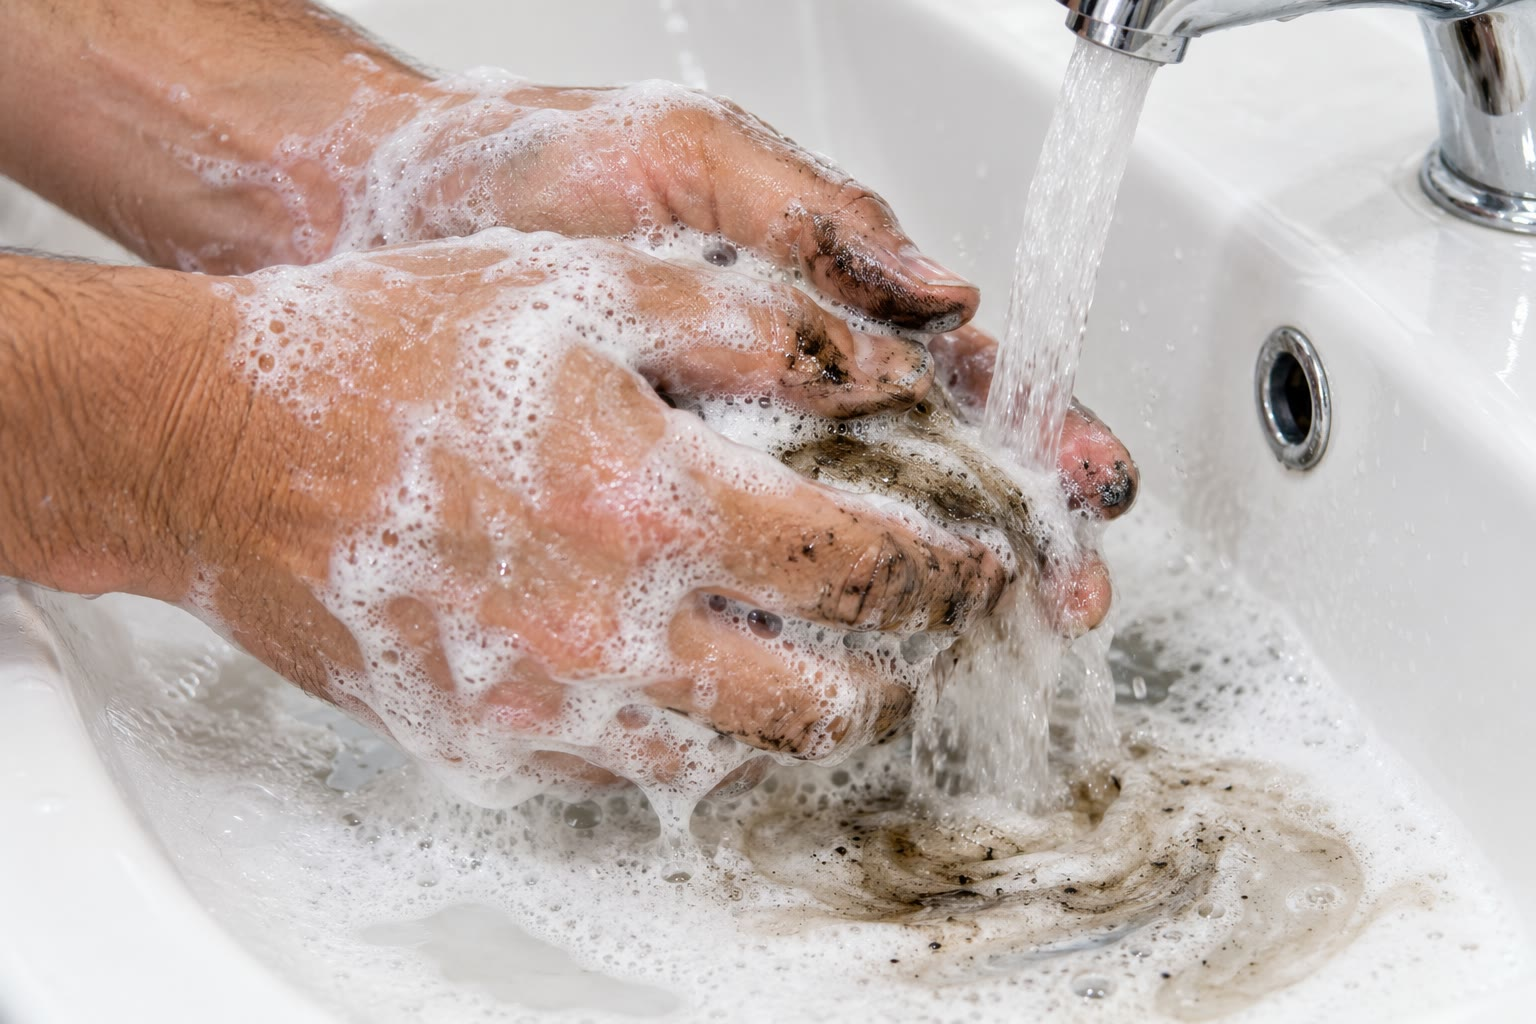
\includegraphics[width=0.48\linewidth]{images/book1/ai/g11-greasy-hands.jpg}

{\small Washing greasy hands: soap carries the grease off in \omterm{def:g11:dissolution:amphiphilic}{micelles}.}
\end{omfigure}

\begin{remark}[Hard water and scum]\label{rem:g11:dissolution:scum}
Hard water contains many calcium \omterm{def:g9:ions:ion}{ions} \ce{Ca^{2+}} and magnesium \omterm{def:g9:ions:ion}{ions}
\ce{Mg^{2+}}, dissolved from the rocks it has run through. With stearate
\omterm{def:g9:ions:ion}{ions} they form a \omterm{def:g9:ions:precipitate}{precipitate} (\cref{ch:g9:ions}), calcium stearate:
\[
  \ce{2C17H35COO- + Ca^{2+} -> Ca(C17H35COO)2(s)} .
\]
This greyish solid is the scum that rings a washbasin, and every soap
\omterm{def:g9:ions:ion}{ion} caught in it is lost for washing: in hard water, soap lathers badly
until enough has been added to \omterm{def:g9:ions:precipitate}{precipitate} all the calcium.
\end{remark}

\begin{omfigure}
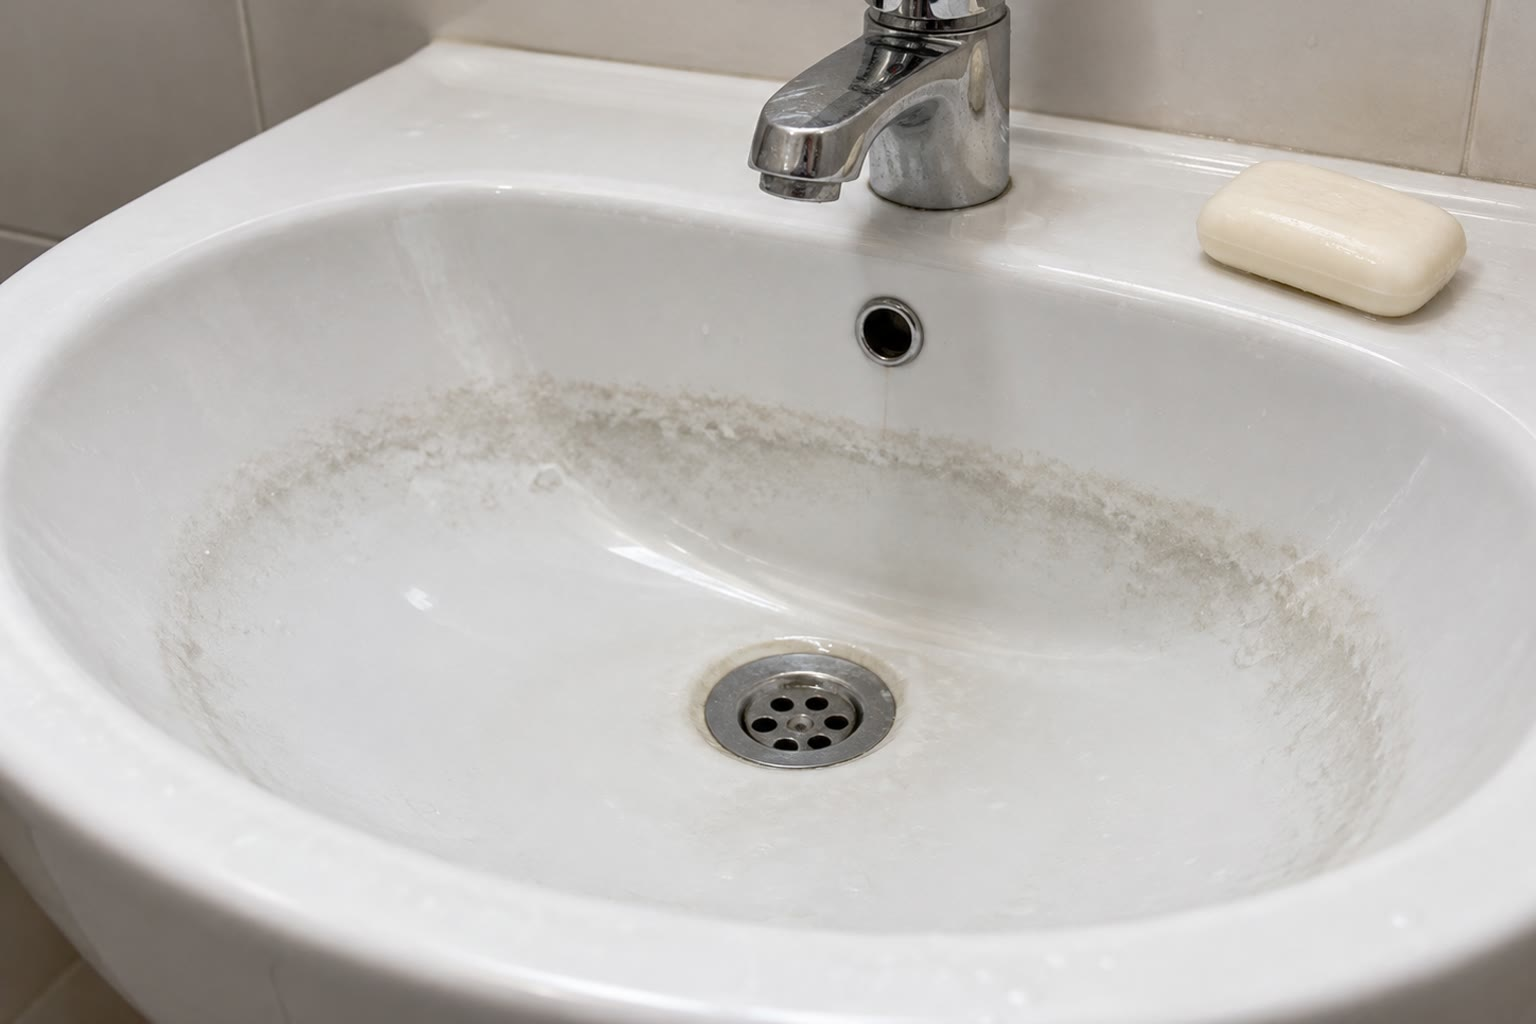
\includegraphics[width=0.45\linewidth]{images/book1/ai/g11-soap-scum.jpg}

{\small Soap scum in a basin: calcium stearate, precipitated by hard
water.}
\end{omfigure}

\section{Exercises}


\begin{exercise}[$\star$]\label{exo:g11:dissolution:1}
Write the dissolution equations in water of sodium chloride \ce{NaCl},
calcium chloride \ce{CaCl2}, sodium sulfate \ce{Na2SO4} and aluminium
chloride \ce{AlCl3}.
\end{exercise}

\begin{exercise}[$\star$]\label{exo:g11:dissolution:2}
A solution of sodium sulfate has $c = \qty{0.050}{mol/L}$. Give the
concentrations of the sodium \omterm{def:g9:ions:ion}{ions} and of the sulfate \omterm{def:g9:ions:ion}{ions}.
\end{exercise}

\begin{exercise}[$\star$]\label{exo:g11:dissolution:3}
What is meant by the \omterm{def:g11:dissolution:solvation}{hydration} of an \omterm{def:g9:ions:ion}{ion}? Which end of a water \omterm{def:g7:atoms-and-molecules:molecule}{molecule}
points towards a \omterm{def:g9:ions:ion}{cation}, which towards an \omterm{def:g9:ions:ion}{anion}? Why?
\end{exercise}

\begin{exercise}[$\star$]\label{exo:g11:dissolution:4}
\qty{2.67}{g} of aluminium chloride are dissolved to make
\qty{200.0}{mL} of solution. Compute the concentration of the solution
and of each \omterm{def:g9:ions:ion}{ion}.
\end{exercise}

\begin{exercise}[$\star$]\label{exo:g11:dissolution:5}
Label each part of the stearate \omterm{def:g9:ions:ion}{ion} as \omterm{def:g11:dissolution:hydrophilic}{hydrophilic} or \omterm{def:g11:dissolution:hydrophilic}{hydrophobic}, and
say why.
\end{exercise}

\begin{exercise}[$\star\star$]\label{exo:g11:dissolution:6}
Which \omterm{def:g6:solutions-and-solubility:solute}{solvent}, water or cyclohexane, would you choose to \omterm{def:g2:mixing-and-dissolving:dissolve}{dissolve}: salt;
candle wax (long hydrocarbon chains); sugar (many \ce{O-H} groups);
iodine? Justify each choice.
\end{exercise}

\begin{exercise}[$\star\star$]\label{exo:g11:dissolution:7}
Ethanol \ce{CH3-CH2-OH} \omterm{def:g2:mixing-and-dissolving:mix}{mixes} with water in all proportions, but hexane
\ce{C6H14} does not \omterm{def:g2:mixing-and-dissolving:mix}{mix} with water. Explain.
\end{exercise}

\begin{exercise}[$\star\star$]\label{exo:g11:dissolution:8}
Look at the \omterm{def:g11:dissolution:amphiphilic}{micelle} figure. Why are the tails inside and the heads
outside? Why do two \omterm{def:g11:dissolution:amphiphilic}{micelles} not merge into one larger drop of grease?
\end{exercise}

\begin{exercise}[$\star\star$]\label{exo:g11:dissolution:9}
A plant scent is dissolved in water. To extract it, a chemist can use
ethanol or cyclohexane. Which one is suitable, and why is the other not
(think of \omterm{def:g6:solutions-and-solubility:miscible}{miscibility})?
\end{exercise}

\begin{exercise}[$\star\star$]\label{exo:g11:dissolution:10}
In the iodine \omterm{def:g10:chemical-species:extraction}{extraction}, why is the cyclohexane layer on top? Which
layer is run off through the tap? Where is the iodine at the end?
\end{exercise}

\begin{exercise}[$\star\star$]\label{exo:g11:dissolution:11}
A blue solution of copper sulfate is shaken with cyclohexane. What
happens to the blue colour? Explain.
\end{exercise}

\begin{exercise}[$\star\star\star$]\label{exo:g11:dissolution:12}
What mass of calcium chloride must be dissolved to make \qty{250.0}{mL}
of a solution in which $[\ce{Cl-}] = \qty{0.300}{mol/L}$?
\end{exercise}

\begin{exercise}[$\star\star\star$]\label{exo:g11:dissolution:13}
A sample of sea water is found to contain \qty{0.010}{mol/L} of calcium
\omterm{def:g9:ions:ion}{ions} and \qty{0.053}{mol/L} of magnesium \omterm{def:g9:ions:ion}{ions}. Explain why ordinary soap lathers
very badly in sea water. How much sodium stearate would be precipitated
by the calcium \omterm{def:g9:ions:ion}{ions} alone of one litre of sea water?
\end{exercise}

\begin{exercise}[$\star\star\star$]\label{exo:g11:dissolution:14}
\qty{100.0}{mL} of sodium chloride solution at \qty{0.20}{mol/L} are
mixed with \qty{100.0}{mL} of calcium chloride solution at
\qty{0.10}{mol/L}. No \omterm{def:g9:ions:precipitate}{precipitate} forms. Compute the concentrations of
\ce{Na+}, \ce{Ca^{2+}} and \ce{Cl-} in the \omterm{def:g6:pure-substances-and-mixtures:mixture}{mixture}, and check that it is
neutral.
\end{exercise}

\begin{exercise}[$\star\star\star$]\label{exo:g11:dissolution:15}
% ledger: sol:I2-water, sol:I2-heptane, rho:heptane
Iodine \omterm{def:g2:mixing-and-dissolving:dissolve}{dissolves} at about \qty{0.3}{g} per litre of water and
\qty{17}{g} per kilogram of heptane. Heptane has a density of about
\qty{0.68}{kg/L}. How many times more iodine can a litre of heptane hold
than a litre of water? What does this mean for an \omterm{def:g10:chemical-species:extraction}{extraction}?
\end{exercise}

\section{Problem: Soap and Hard Water}

\begin{problem}[{Weekend problem --- how much soap does a bath of hard
water waste as scum?}]
\label{pb:g11:dissolution:1}
% ledger: aw:Ca, aw:Mg, aw:C, aw:H, aw:O, aw:Na
A tap water contains \qty{120}{mg} of calcium \omterm{def:g9:ions:ion}{ions} and \qty{24}{mg} of
magnesium \omterm{def:g9:ions:ion}{ions} per litre. A bath is filled with \qty{150}{L} of it, and
the bather uses a soap made of sodium stearate, \ce{C17H35COONa}.

\medskip
\noindent\textbf{Part I --- What is in the water.}
\begin{enumerate}
  \item Where do the calcium and magnesium \omterm{def:g9:ions:ion}{ions} of tap water come from?
  \item Compute the \omterm{def:g10:concentration-and-dilution:molar-concentration}{molar concentrations} of the calcium \omterm{def:g9:ions:ion}{ions} and of the
        magnesium \omterm{def:g9:ions:ion}{ions}.
  \item The calcium \omterm{def:g9:ions:ion}{ions} are accompanied by hydrogencarbonate \omterm{def:g9:ions:ion}{ions},
        \ce{HCO3-}, as if calcium hydrogencarbonate \ce{Ca(HCO3)2} had
        been dissolved. Write that dissolution equation, and deduce the
        concentration of hydrogencarbonate \omterm{def:g9:ions:ion}{ions} that goes with the
        calcium.
  \item What amount of calcium \omterm{def:g9:ions:ion}{ions} does the bath contain?
\end{enumerate}

\medskip
\noindent\textbf{Part II --- The soap.}
\begin{enumerate}[resume]
  \item Compute the \omterm{def:g10:the-mole:molar-mass}{molar mass} of sodium stearate.
  \item Write its dissolution equation in water.
  \item Which part of the stearate \omterm{def:g9:ions:ion}{ion} is \omterm{def:g11:dissolution:hydrophilic}{hydrophilic}, which
        \omterm{def:g11:dissolution:hydrophilic}{hydrophobic}? Why is it called \omterm{def:g11:dissolution:amphiphilic}{amphiphilic}?
  \item Describe a \omterm{def:g11:dissolution:amphiphilic}{micelle}, and explain how it removes grease from the
        skin.
  \item Why must soap be dissolved in water, not in oil, to wash?
\end{enumerate}

\medskip
\noindent\textbf{Part III --- Scum.}
\begin{enumerate}[resume]
  \item Write the equation of the \omterm{def:g9:ions:precipitate}{precipitation} of calcium stearate.
        Check that it is balanced in charge.
  \item Fill the \omterm{def:g10:reaction-progress-table:extent}{progress table} for \qty{1.00}{L} of the tap water and an
        excess of stearate \omterm{def:g9:ions:ion}{ions}. Which \omterm{def:g7:chemical-reactions:reactant}{reactant} is limiting?
  \item What amount of stearate \omterm{def:g9:ions:ion}{ions} is lost per litre to the calcium?
  \item Compute the \omterm{def:g10:the-mole:molar-mass}{molar mass} of calcium stearate, and the mass of scum
        formed per litre.
  \item Magnesium stearate \omterm{def:g9:ions:precipitate}{precipitates} in the same way. What amount of
        stearate do the magnesium \omterm{def:g9:ions:ion}{ions} take per litre?
\end{enumerate}

\medskip
\noindent\textbf{Part IV --- The bath.}
\begin{enumerate}[resume]
  \item What amount of stearate \omterm{def:g9:ions:ion}{ions} does the calcium of the whole bath
        \omterm{def:g9:ions:precipitate}{precipitate}?
  \item What mass of soap is that?
  \item Adding the magnesium, what mass of soap is wasted in all?
  \item Bars of soap weigh about \qty{100}{g}. How many bars does the
        calcium alone take?
  \item State the final answer: what mass of soap does the calcium of one
        \qty{150}{L} bath of this water waste as scum?
\end{enumerate}
\end{problem}
